% Book pp. 172-175 (PDF pp. 173-176).  The numbering is the book's own.
\section*{Review Questions}
\booknote[S4-15]{the book numbers the questions 1 to 25, but several single
problems are split over two numbers (1/2, 6/7, 10/11, 12/13, 14/15 and 24/25),
and question 1 g is the last sentence of 1 f. The answer key numbers the same
problems 1 to 19.}

\begin{enumerate}[leftmargin=*, widest=25]
\item[1.] The diagram below shows the graph of three circles, P, Q and R.
\item[2.] Use it to answer the questions\textbf{.}
\begin{center}
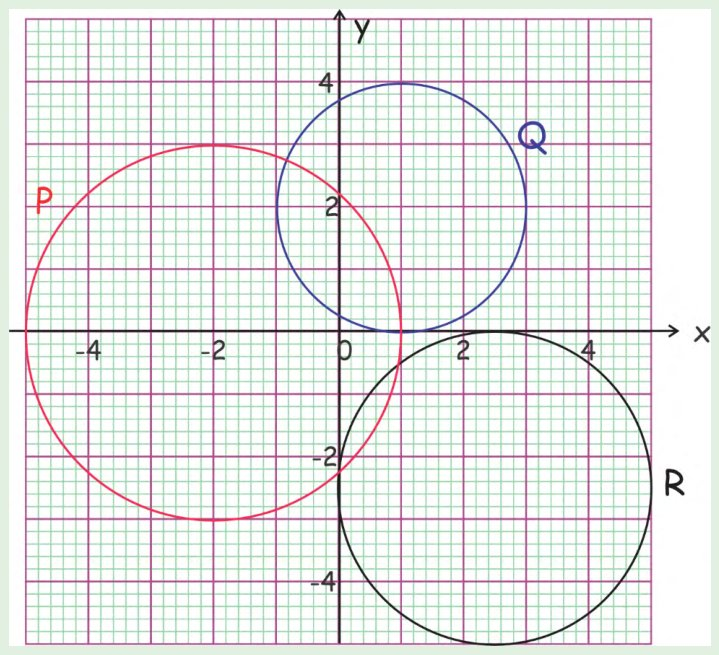
\includegraphics[width=0.6\linewidth]{figures/rq4-1.jpg}
\end{center}
\begin{enumerate}
  \item[a.] State the coordinates of the centre of P, Q and R.
  \item[b.] Find the radii of circles P, Q and R
  \item[c.] Write the equation of circle R in general form
  \item[d.] Write the equation of circle P in the standard form
  \item[e.] Write the equation of circle Q in the standard form
  \item[f.] Find the perimeter of the triangle formed by the centres of the three
  circles.
  \item[g.] Give your answer correct to three significant figures.
\end{enumerate}

\item[3.] Write the general form of the circle equation with the following properties.
\begin{enumerate}
  \item[a.] Centre (1, -1) and radius 7
  \item[b.] Centre (-2, 1) and radius 5
  \item[c.] Centre (0, -3) and radius 2
  \item[d.] Centre (-3, -4) and radius 8
\end{enumerate}

\item[4.] The diagram shows the graph of circles A, B and C.

Use them to answer the following questions.
\begin{center}
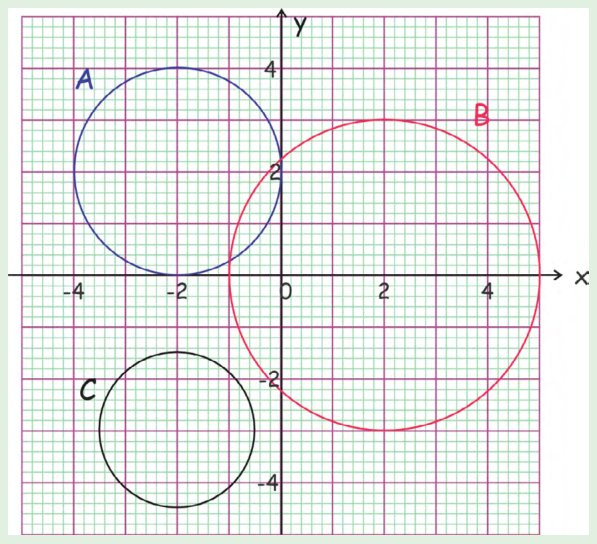
\includegraphics[width=0.5\linewidth]{figures/rq4-4.jpg}
\end{center}
\begin{enumerate}
  \item[a.] Write the equation of each circle in the general form
  \item[b.] Find the perimeter of the triangle formed by the centres of the circle.
  Leave your answer in surd form.
\end{enumerate}

\item[5.] A TV remote has a range of 8m in all directions. If the TV is 5m East and
3m South, write an equation to represent the area within which the TV
receives signals from the remote. Can the TV receive signals from the
remote if the remote is located 2m West? Justify your response.

\item[6.] An Uber driver operates within 30km of a post office at all angles. His
house is 5km West and 12km south of a post office.
\item[7.] \mbox{}
\begin{enumerate}
  \item[a.] Write an equation to represent the driver's travel boundary from the
  post office using the driver's house as the origin. Leave your equation
  in standard form.
  \item[b.] Find the furthest distance between the driver's house and his travel
  boundary.
  \item[c.] Find the shortest distance between the driver's house and the driver's
  travel boundary.
\end{enumerate}

\item[8.] Write the general equation of a circle with:
\begin{enumerate}
  \item[a.] Centre $(4, -1)$ and radius $\sqrt{11}$.
  \item[b.] Centre $(-2, -3)$ and radius $2\frac{1}{2}$
  \item[c.] Centre $(0, -3)$ and radius $\frac{1}{3}$
  \item[d.] Centre $\left(\frac{1}{2}, -1\right)$ and radius $1\frac{1}{2}$
\end{enumerate}

\item[9.] Write each of the following circles in the standard form. Also, state the
centre and radius of each circle.
\begin{enumerate}
  \item[a.] $x^2 + y^2 - 2x + 2y - 47 = 0$
  \item[b.] $x^2 + y^2 + 6y = 0$
  \item[c.] $x^2 + y^2 - 12x - 64 = 0$
  \item[d.] $x^2 + y^2 + 4x - 8y + 4 = 0$
  \item[e.] $2x^2 + 2y^2 - 2x - 2y - 7 = 0$
  \item[f.] $3x^2 + 3y^2 + 12x - 2y + 4 = 0$
\end{enumerate}

\item[10.] The endpoints of the diameter of a circle are (0, 5) and (0, -7).
\item[11.] Find the
\begin{enumerate}
  \item[a.] radius and centre of the circle
  \item[b.] general equation of the circle.
\end{enumerate}

\item[12.] The endpoints of the diameter of a circle are (6, 0) and (-2, 0).
\item[13.] Find the
\begin{enumerate}
  \item[a.] radius and centre of the circle
  \item[b.] general equation of the circle.
\end{enumerate}

\item[14.] The endpoints of the diameter of a circle are (-4, 3) and (4, -3).
\item[15.] Find the
\begin{enumerate}
  \item[a.] radius and centre of the circle
  \item[b.] general equation of the circle.
\end{enumerate}

\item[16.] In each of the following questions, coordinates of three points are provided.
Write the general equation of the circle that satisfies all three points. State
the centre and radius of the resulting circle.
\begin{enumerate}
  \item[a.] $(-5, 0)$, $(-1, -4)$ and $(-1, 4)$
  \item[b.] $(6, -1)$, $(3, -4)$ and $(0, -1)$
\end{enumerate}

\item[17.] Find the equations of the line tangent and normal to the circle.
\begin{enumerate}
  \item[a.] $x^2 + y^2 = 100$ at point $(-8, -6)$
  \item[b.] $x^2 + y^2 = 49$ at point (7, 0)
  \item[c.] $x^2 + y^2 - 2x - 24 = 0$ at (1, -5)
\end{enumerate}

\item[18.] Find the length of the tangent from the point:
\begin{enumerate}
  \item[a.] (-8, 6) to the circle $x^2 + y^2 - 25 = 0$, leave your answer in surd form
  \item[b.] (3, 6) to the circle $x^2 + y^2 - 4y - 5 = 0$
  \item[c.] $(7, -3)$ to the circle $x^2 + y^2 + 10x - 4y + 13 = 0$, leave your answer
  in surd form
  \item[d.] $\left(5, -\frac{1}{2}\right)$ to the circle $4x^2 + 4y^2 + 12x + 4y - 15 = 0$
\end{enumerate}

\item[19.] The diagram below shows a graph of a circle. Line BA is a tangent to the
circle at B.
\begin{center}
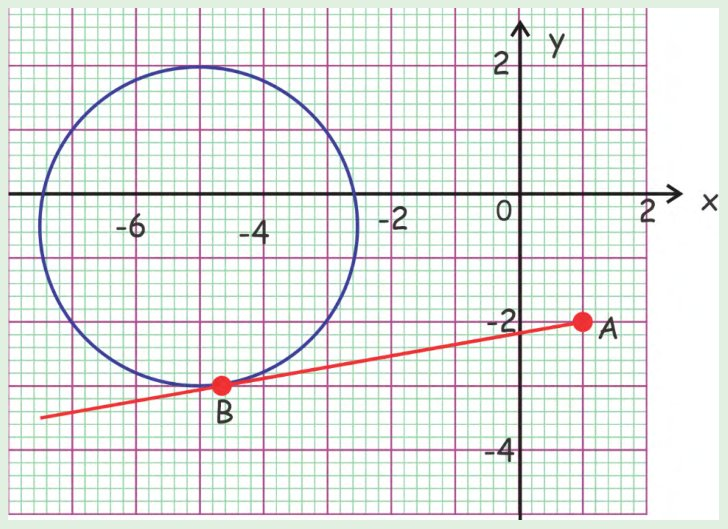
\includegraphics[width=0.6\linewidth]{figures/rq4-19.jpg}
\end{center}
\begin{enumerate}
  \item[a.] Find the equation of the circle.
  \item[b.] Find $|$AB$|$, leave your answer in surds
\end{enumerate}

\item[20.] Calculate the equation of all points equidistant from A(-4, 0) and B(2, 8))

\item[21.] Find the equation of the locus of points which moves so that its distance
from the lines $3y - x = 0$ and $x - 3y = 0$ is the same.
\booknote[S4-16]{$3y - x = 0$ and $x - 3y = 0$ are the same line, so as printed
the question has no meaningful answer; the answer key gives $y - x = 0$.}

\item[22.] Find the locus of point R(x, y) that is always 2 units from the line $x + 5 =
0$

\item[23.] If P(-2, 1) and Q(4, -1) are two fixed points and A($x$, $y$) moves such that
$|$AP$|$:$|$AQ$| = 2$:1. Find the equation of the locus\textbf{.}

\item[24.] A point A($x$, $y$) moves so that AC and AD are perpendicular. C(-2, 0) and
D(6, 4).
\item[25.] Find the equation of the locus A.
\end{enumerate}
